\section{Grundlagen}
\label{sec:basics}

Im Folgenden werden \textit{Markov Entscheidungsprozesse}, ein fundamentales Modell im RL, vorgestellt. Anschließend gehen wir kurz auf das \textit{Sparse Reward Problem} ein.

\subsection{Markov Entscheidungsprozesse}
\label{sec:reinforcement}
\begin{figure}[h]
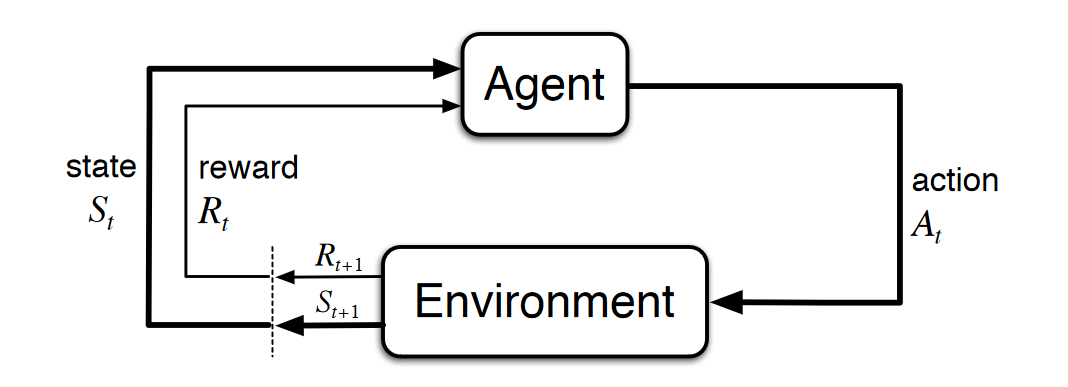
\includegraphics[width=\textwidth, keepaspectratio=true]{images/mdp.png}
\caption{Typischer Reinforcement Learning Zyklus} \label{img:rl_cycle}
\source{\cite{deeplizard_markov_decision_processes}}
\end{figure}
Das wohl elementarste Modell im RL sind Markov Entscheidungsprozesse (MDPs von engl. \textit{Markov Decision Processes}), hier erklärt nach \cite{deeplizard_markov_decision_processes}.

Ein MDP besitzt einen Entscheidungsträger, den so genannten \textit{Agenten} (im Folgenden auch als \textit{Aktor} bezeichnet), welcher mit seiner Umgebung (dem \textit{Environment}) interagiert. Diese Interaktion findet sequentiell statt. In jedem Zeitschritt $ t $ verfügt der Agent über eine Repräsentation seiner Umgebung, den Zustand oder auch \textit{State} $ S_t $. Aufgrund der dem Agenten vorliegenden Information wählt dieser eine Aktion $ A_t $. Dies führt dazu, dass das Environment in einen neuen Zustand $ S_{t+1} $ überführt wird. Außerdem erhält der Aktor von der Umgebung eine Belohnung $ R_{t+1} $, den \textit{Reward}.

Wie in \ref{img:rl_cycle} dargestellt findet dieser Prozess in einem andauernden Zyklus statt. Ziel des Agenten ist es, die Summe aller Rewards, die er für die Ausführung von Aktionen bekommt, zu maximieren. Sprich der Agent will nicht nur den folgenden Reward, sondern viel eher die Gesamtheit aller Rewards, die er auf Dauer bekommt, maximieren.

\subsection{Sparse Reward Problem}
\label{sec:sparse_reward}
Ein zentrales Problem im RL ist nach \cite{hare2019dealing} der Umgang mit Umgebungen, in denen Belohnungen nur spärlich vorhanden sind. Eine Reihe von Belohnungen, von denen die meisten nicht positiv sind, wird als \textit{Sparse Reward} bezeichnet. Diese machen es für RL-Algorithmen sehr schwer, eine Reihe von Aktionen mit einem weit entfernten Reward zu verbinden. In extremen Fällen findet der Agent eventuell gar keine Belohnung und wird so niemals lernen, wie er die gegebene Aufgabe bewältigt \cite{hare2019dealing}.

Um das Problem zu umgehen müssen die Belohnungen im traditionellen RL sehr sorgfältig durchdacht sein. Dies erfordert viel Zeit und Verständnis für die Umgebung. Besser währe es also, wenn der Agent mit Sparse Rewards umgehen kann und die Ziele somit abstrakter und langfristiger definiert werden können, wodurch komplexere Aufgaben behandelt werden können \cite{hare2019dealing}.

Um dies zu erreichen existieren bereits mehrere Ansätze, von denen zwei im Folgenden vorgestellt werden.